% Appendix
\clearpage

\chapter*{Appendix}
\addcontentsline{toc}{chapter}{Appendix}

\appendix

\begin{enumerate}
\item Licensing Information
\item DYNAMO Scripting Language
\item Information for Developers
\end{enumerate}

\section{Licensing Information}
\index{licensing}
This program is free software: you can redistribute it and/or modify it under the terms of the GNU General Public License as published by the Free Software Foundation, either version 3 of the License, or (at your option) any later version.

This program is distributed in the hope that it will be useful, but WITHOUT ANY WARRANTY; without even the implied warranty of MERCHANTABILITY or FITNESS FOR A PARTICULAR PURPOSE.  See the GNU General Public License for more details.

You should have received a copy of the GNU General Public License along with this program.  

If not, see "http://www.gnu.org/licenses".
\bigskip


\subsection{GNU General Public License}

\index{GNU GPL}
\input gnuGPL

\subsection{GNU Lesser General Public License}

\index{GNU LGPL}
\input gnuLGPL

\section{DYNAMO Scripting Language}
\label{dynamo appendix}
Content in this section is adapted from the DYNAMO Reference Manual Edition 1.9.7 and the Dynamical Language Reference Manual Edition 1.0.0, both written by Ivan Raikov at the Georgia Institute of Technology in 2005.

\subsection{Using DYNAMO with RTXI}

DYNAMO models can be edited using your choice of text editor and compiled into RTXI models from within RTXI by selecting the menu item Modules $\rightarrow$ Load DYNAMO Module. The DYNAMO model is first parsed into C++ header and implementation files, which are then compiled into shared object libraries similar to other RTXI modules. After the initial compilation, the model can be loaded using the menu item Modules $\rightarrow$ Load User Module, without repeating the parsing step. User-specified variable names and equations are not preserved in the resulting CPP files so changes to your model should be made to the original DYNAMO module. If changes are made, the DYNAMO module should be re-parsed and compiled. If you started RTXI from the terminal, the progress of the parsing and compilation steps, as well as any errors in your DYNAMO  syntax, will be displayed there.

There should already be a working DYNAMO script located in /usr/bin, but the following instructions will allow you to compile the DYNAMO translation script from scratch in Ubuntu 8.10/9.04/9.10. 
\begin{example}
\$ sudo apt-get install mlton\\
\$ cd /rtxi/dynamo\\
\$ mllex dl.lex\\
\$ mlyacc dl.grm\\
\$ mlton dynamo.mlb\\
\$ sudo cp dynamo /usr/bin
\end{example}

\subsection{Running DYNAMO from the terminal}

The DYNAMO translator is run with the command \texttt{dynamo} followed by names of files to be translated, and options that specify the type of output. For example:

\begin{example}
  dynamo --matlab  morris-lecar.dynamo
\end{example}

This command specifies that the DYNAMO translator should translate file \texttt{morris-lecar.dynamo} to MATLAB code. Below is a summary of all options accepted by the DYNAMO translator:

\begin{table}[htdp]
\caption{DYNAMO translator options}
\begin{center}
\vspace{.5cm}
\begin{tabular}{ll}
\textbf{Options(s)} & \textbf{Description}\\
\texttt{-h,  --help} & describes the options\\
\texttt{-version, --release} & show version information\\
\texttt{-o [FILE],  --output[=FILE]} & set the prefix of output file(s)\\
\texttt{-e [FILE],  --error-output[=FILE]} & redirect error messages\\
\texttt{--eqdfg[=FILE]} & output the equation DFG\\
\texttt{--exdfg[=FILE]} & output the expression DFG\\
\texttt{-r [FILE],  --mrci[=FILE]} & output MRCI model\\
\texttt{-x [FILE],  --rtxi[=FILE]} & output RTXI model\\
\texttt{-m [FILE],  --matlab[=FILE]} & output Matlab model\\
\texttt{--simulink[=FILE]} & output Simulink model\\
\end{tabular}
\end{center}
\label{default}
\end{table}%

\subsection{DYNAMO Syntax}\index{DYNAMO, syntax}

A \emph{model description} describes the dynamical system to be
studied. It consists of \emph{declarations} and \emph{equations}, which
have a certain mathematical meaning, and are not to be confused with
assignment statements in programming languages. These equations do not
have to be entered in any particular order; they are automatically
sorted by the translator so that functions are computed before the
state equations that use them.

\subsubsection{Concepts}

A \emph{user-visible quantity} is something the user can access, change
(provided that it makes sense), and which may have a documentation
associated with it. DYNAMO allows all user-visible quantities to be
manipulated by the user, and in that sense it does not distinguish
between quantities with different mathematical meanings (such as
constants, states, functions, etc.)

The DYNAMO model description language is always case sensitive. The name
`A' is different from `a'. The language has a set of
reserved words, which are always written in capital letters.

The names given to user-visible quantities must obey the following
rules: an identifier consists of a sequence of alpha-numerical
characters, the first of which is a character, and the underscore
`\_' is counted as a character.

Once an identifier is used to declare a state, parameter etc., it
may not be used for any other purpose.

Comments may be written anywhere. The syntax is as in the C and C++
programming languages: either enclosed between `/*' and
`*/', or from `//' and to end-of-line.

\subsubsection{Structure of a DYNAMO Model}

A DYNAMO model file consists of a declaration section followed by a time block. The declaration section consists of a number of declarations. Every declaration is ended by a semicolon. The first declaration has to be a declaration of the model, such as:

\begin{example}
  MODEL \emph{system\_name}
\end{example}

where \emph{system\_name} follows the rules for an identifier name.

After the system declaration, there follow a number of declarations of states, parameters, and functions. There has to be exactly one time declaration.

\subsubsection{Declarations}

The declaration section specifies the names and initial values of all
quantities in the dynamical system. Every declaration is ended by a
semicolon. The first declaration has to be a declaration of the
system, which simply states the name of the model for informative
purposes.  

After the model name, there follows a number of declarations for
\emph{parameters}, \emph{states}, \emph{external states} and
\emph{functions}.  The declaration section concludes with exactly one
\emph{time declaration}.

\emph{Parameters} are constants during integration. The syntax 
for declaring a parameter is
\begin{example}
        PARAMETER \emph{name} = \emph{default\_value} ``\emph{description}''
\end{example}

where \emph{description} is optional. The description string is there
for convenience and is not read by any program. It is always optional,
so it can be omitted. 

\emph{Vector parameters} are constant vector values. The syntax  
for declaring a vector parameter is
\begin{example}
       VECTOR PARAMETER \emph{name} = ( \emph{element0}, \emph{element1}, ... ) ``\emph{description}'';
\end{example}

The parameter declared in this manner will have a vector value
initialized with the scalar elements supplied by the user. The size of
the vector is equal to the number of initialization elements given,
and remains constant throughout the simulation.

\emph{States} are the components of the dynamical system whose values
change over time and are computed by a difference or differential
equation.  There are several different kinds of states. \emph{Scalar
states} can only contain a scalar value and are declared with the
keyword \texttt{STATE}:

\begin{example}
        STATE \emph{name} = \emph{initial condition} ``\emph{description}'';
\end{example}

where \emph{name} is the name of the state as the user sees it and
\emph{initial condition} is the default initial condition, a real
constant.

For example, in the following declaration,

\begin{example}
        STATE x = 0.1 "gating variable for inward conductance";
\end{example}

\texttt{x} is the name of the state, and 0.1 is the default initial
condition.

The above declaration will create a state variable which is integrated
using an equation in the time block, described later in this
section. The default method for integration is Euler's method. DYNAMO
also supports a method we call \emph{multiply-add-update}, in which the
state variable being integrated is multiplied and added with the values
returned by two functions dependent on \texttt{dt}.  The method of
integration can be specified with the \texttt{METHOD} attribute of the
state definition, as follows:

\begin{example}
        STATE \emph{name} = \emph{initial condition} METHOD \emph{method\_name};
\end{example}

where \texttt{method\_name} can be either \texttt{euler} or \texttt{mau},
indicating Euler or multiply-add-update, respectively. Thus, our
example can be changed to:

\begin{example}
        STATE x = 0.1 METHOD "mau" 
                "gating variable for inward conductance";
\end{example}

\emph{Integer states} are exactly the same as scalar states, only they
can only have an integer initial value, and only the integer part of
their equation is assigned to them.

\emph{Vector states} are states that can only hold a vector value of
fixed size:

\begin{example}
        VECTOR STATE \emph{name} = ( \emph{initial0}, \emph{initial1}, ... ) ``\emph{description}'';
\end{example}

The state declared above will have an initial value that is a vector
initialized with the scalar elements supplied by the user. The size of
the vector is equal to the number of initialization elements given,
and remains constant throughout the simulation. Vector states cannot
be assigned equations that return a vector of size different than that
of their initial value.

\emph{Discrete states} are state quantities whose value can only be one
of several enumerated (discrete) values:

\begin{example}
        DISCRETE STATE status = ( inactive, threshold, active ) ``\emph{description}'';
\end{example}

The names of the possible values are supplied by the user, and are
implicitly assigned integer values starting from one and incrementing
by one. These default integer values can be overridden as follows: 

\begin{example}
        DISCRETE STATE status = ( inactive=5, threshold=10, active=20 );
\end{example}

\emph{External states} are states whose value is either obtained through
the data acquisition board (\emph{external input}), or whose value is
being output to the data acquisition board (\emph{external output}). They
are declared as: 

\begin{example}
        EXTERNAL INPUT Vin1, Vin2;
        EXTERNAL OUTPUT Vout;
\end{example}

The input state can then be used in equations and expressions; the
output state may not be used in expressions, and it must be assigned a
value.  The values of these external state variables are in terms of
the units provided by the data acquisition board, usually volts. The
order in which external input and output states are declared
determines their assignment to physical channels of the data
acquisition board.  For example, in the above declaration, state
\emph{Vin1} will be assigned to input channel 0, and state \emph{Vin2}
will be assigned to input channel 1. Had they been declared in reverse
order, then state \emph{Vin1} would have been assigned to input channel
1, and state \emph{Vin2} would have been assigned to input channel 0.

\emph{Functions} are quantities that are statically dependent on other
quantities in the system---unlike state equations, their equations are
not permitted to use the previously computed value of the
quantity. There are \emph{scalar functions} which return a scalar
value, and \emph{vector functions} which return a vector value.

\begin{example}
        STATE FUNCTION \emph{name} "\emph{description}";
\end{example}

and

\begin{example}
        VECTOR FUNCTION \emph{name} "\emph{description}";
\end{example}

For all systems, there is only one ``time'', to be declared with the
declaration \texttt{TIME}. The syntax is

\begin{example}
        TIME \emph{name};
\end{example}

The time variable that was declared with the above statement can be
used anywhere in the model equations. Its value is a real number that
represents the number of milliseconds elapsed since the beginning of
the simulation. At each computational step it is incremented by
\texttt{dt}.

The declarations section may also contain \emph{function lookup tables}.
These define a function whose value is computed by interpolating
datapoints in a table indexed by a state variable.  This feature can
greatly speed up computation.  An example lookup table definition is
shown below.

\begin{example}
        TABLE FUNCTION F1(v) = (1 + tanh(v)), 
                       LOW = -10.1, HIGH = 10.1, STEP = 0.1, 
                       DEPENDENCY = F2;
\end{example}

The various syntactic components of this statement have the following
meanings: 
\begin{itemize}
\item \texttt{TABLE FUNCTION F(v)}---declaration of a function called \texttt{F1}, which has one argument, \texttt{v}. Note that the function argument is only to be used inside the function expression; it is \emph{NOT} (or doesn't have to be) the name of the variable used for looking up datapoints in the function table.
\item \texttt{(1 + tanh(v))}---the actual function expression. See Appendix \ref{DYNAMOtimeblock}, for details on arithmetic expressions in DYNAMO. Note the use of our function argument.
\item \texttt{LOW=-10.1,HIGH=10.1,STEP=0.1}---the lower boundary of interpolation datapoints, the upper boundary of interpolation datapoints, and the interval for datapoints between the two boundaries. DYNAMO will compute datapoints starting at the lower boundary and reaching to the upper boundary using the given step.
\item \texttt{DEPENDENCY=F2}---the name of the dependency. This can be a function, state, parameter, etc. At run-time, the value of this quantity will be computed first, then it will be given as an input to the interpolation function.
\end{itemize}

\subsubsection{Time Blocks}
\label{DYNAMOtimeblock}

A time block describes the equations which are in effect during the
named time. Dynamic equations are all in the \texttt{AT TIME t}-block
(assuming that the system time is called \texttt{t}).  The equations in
a time block are, if possible, sorted in order so they can be
sequentially executed. If the equations contain a circular dependence,
the sorting will fail. The DYNAMO translator can not solve algebraic
loops (It can be claimed that in this case, the user has not written
complete and consistent equations for the system). Other sanity tests
(like that every derivative is assigned to exactly once) are also
performed.

Function expressions are specified in the following manner:

\begin{example}
        f1 = sin((1 + a) / 5)
\end{example}

The above statement will specify that at each iteration, the quantity
\emph{f1} will have the value computed with the given
expression. \emph{f1} then can be used in the expressions of other
functions, differential equations, etc:

\begin{example}
        f2 = sin(f1 * 12)
\end{example}

On the right hand side, almost any scalar C expression is allowed: The
exponential operator, denoted either \emph{$\ast\ast$} or \emph{$^{\wedge}$}, has been
added to the C syntax.  The equation, which may run over several
lines, is terminated with a semicolon. Further, the sequencing
operator (the comma) is not allowed, since an expression sequence can
hardly be an ``equation''. See \ref{Expressions and Operators in the
System Description Language}, for a complete description of the
possible arithmetic expressions.

Standard mathematical functions are available with their usual
names (log, cos, atan, etc@dots{}). See \ref{Mathematical Functions in
the System Description Language}, for a list of all DYNAMO-supported mathematical
functions. 

Differential equations are specified in the following form:
\begin{example}
        d(\emph{state}) = \emph{right-hand side};
\end{example}
Here \texttt{d( )} denotes the differential operator, and \texttt{d(x)}
should here be interpreted as ${dx/dt}$.  On the right-hand side,
the same rules apply as for function expressions.

In cases where the desired method of integration requires more than
one equation (such as the multiply-add-update method), the equations are
written as a comma-separated list enclosed in brackets. Thus:
\begin{example}
        d(\emph{state}) = [ \emph{exp1}, \emph{exp2} ];
\end{example}

For difference equations, the dynamic equation takes the form
\begin{example}
        q(x) = right-hand side;
\end{example}
Here we think of \texttt{q} as the forward shift operator: \texttt{q(x(t)) =
x(t + 1)}. 

A time block may also contain a block of arbitrary C code. It should
occur first in the time block. It will be executed before the
equations. There is presently no possibility to put raw C code
\emph{after} the equations are executed. (However, one way to
circumvent this would be to use function calls, e.g. of the type
\emph{d(z) = f(z) + function();} where \texttt{function} always returns
\texttt{0}.)

Declarations of states etc.: are also allowed in the time block, as
long as a quantity is declared before it is referenced. This feature
is necessary for certain machine generated system descriptions (e.g.:
using macros).  It is not the recommended practice to take advantage
of it in manually written system descriptions.

One \emph{time} is predefined: \texttt{START}. \texttt{AT TIME START}
contains equations and/or C-code to be executed before the main
integration. For example, functions can be set to their initial values
in this section. If an error is detected the C statement \emph{return
-1;} should be executed. This will stop the simulation.

Dynamic equations (differential equations and difference equations)
are only allowed in the \texttt{AT TIME t} block. Algebraic equations
may occur only in the \texttt{AT TIME t} and the \texttt{AT TIME START}
block.

\subsubsection{Expressions and Operators in the Modeling Language}
\label{Expressions and Operators in the System Description Language}

An \emph{expression} is any sequence of operators and operands in the C
programming language that produces a value. The simplest expressions
are parameter, function, and state names, which yield values
directly. Other expressions combine operators and subexpressions to
produce values.

An expression within parentheses has the same value as the expression
without parentheses would have. Any expression can be delimited by
parentheses to change the precedence of its operators.

All declared quantities can be used in conjunction with C operators to
create more complex expressions. The following table presents the set
of C operators.

\begin{fullpage}
\begin{table}[htdp]
\caption{Expressions and Operators in DYNAMO}
\begin{center}
\vspace{.5cm}
\begin{tabular}{ccl}
\textbf{Operator} & \textbf{Example} & \textbf{Description/Meaning}\\
   \texttt{+} $\left[unary\right]$    &  +a       & Value of \emph{a}\\
   \texttt{-} $\left[unary\right]$    &  -a       & Negative of \emph{a}\\
   \texttt{$\sim$}            &  $\sim$a       & One's complement of \emph{a}  \\
   \texttt{++} $\left[prefix\right]$  &  ++a      & The value of \emph{a} afte increment by one\\
   \texttt{++} $\left[postfix\right]$ & a++       & The value of \emph{a} before increment by one\\
   \texttt{--} $\left[prefix\right]$  & --a   & The value of \emph{a} after decrement by one\\
   \texttt{--} $\left[postfix\right]$ & a--   & The value of \emph{a} before decrement by one\\ \\

   \texttt{+} $\left[binary\right]$     & a + b   & \emph{a} plus \emph{b}\\
   \texttt{-} $\left[binary\right]$     & a - b   & \emph{a} minus \emph{b}\\
   \texttt{*} $\left[binary\right]$     & a * b   & \emph{a} times \emph{b}\\
   \texttt{/}              & a / b   & \emph{a} divided by \emph{b}\\
   \texttt{\%}              & a \% b   & Remainder of \emph{a}/\emph{b}\\
   \texttt{>>}             & a \texttt{>>} b  & \emph{a}, right-shifted \emph{b} bits \\
   \texttt{<<}             & a\texttt{<<} b  & \emph{a}, left-shifted \emph{b} bits \\ \\

   \texttt{<}              & a \texttt{<} b   & 1 if \emph{a} < \emph{b}; 0 otherwise       \\
   \texttt{>}              & a \texttt{>} b   & 1 if \emph{a} > \emph{b}; 0 otherwise           \\ 
   \texttt{<=}             & a \texttt{<}= b  & 1 if \emph{a} <= \emph{b}; 0 otherwise           \\
   \texttt{>=}             & a \texttt{>}= b  & 1 if \emph{a} >= \emph{b}; 0 otherwise           \\
   \texttt{==}          & a == b  & 1 if \emph{a} equal to \emph{b}; 0 otherwise \\
   \texttt{!=}             & a != b  & 1 if \emph{a} not equal to \emph{b}; 0 otherwise \\ \\

   \texttt{\&} $\left[binary\right]$     & a \& b   & Bitwise AND of \emph{a} and \emph{b}       \\         
   \texttt{|}              & a $|$ b   & Bitwise OR of \emph{a} and \emph{b}                 \\
   \texttt{$^{\wedge}$}              & a $^{\wedge}$ b   & Bitwise XOR (exclusive OR) of \emph{a} and \emph{b} \\
   \texttt{\&\&}             & a \&\& b  & Logical AND of \emph{a} and \emph{b} (yields 0 or 1)  \\
   \texttt{||}             & a $||$ b  & Logical OR of \emph{a} and \emph{b} (yields 0 or 1)         \\
   \texttt{!}              & !a      & Logical NOT of \emph{a} (yields 0 or 1)        \\ \\

?: & a ? e1 : e2 & Expression \emph{e1} if \emph{a} is nonzero; Expression \emph{e2} if \emph{a} is zero\\

   \texttt{=}              & a = b        & a, after \emph{b} is assigned to it            \\
   \texttt{+=}             & a += b       & \emph{a} plus \emph{b} (assigned to \emph{a})         \\        
   \texttt{-=}            & a -= b       & \emph{a} minus \emph{b} (assigned to \emph{a})      \\          
   \texttt{*=}             & a *= b       & \emph{a} times \emph{b} (assigned to \emph{a})         \\       
   \texttt{/=}             & a /= b       & \emph{a} divided by \emph{b} (assigned to \emph{a})    \\                  
   \texttt{\%=}             & a \%= b       & Remainder of \emph{a}/\emph{b} (assigned to \emph{a})     \\    
   \texttt{>>=}            & a \texttt{>>}= b      & \emph{a}, right-shifted \emph{b} bits (assigned to \emph{a})  \\
   \texttt{<<=}            & a \texttt{<<}= b      & \emph{a}, left-shifted \emph{b} bits (assigned to \emph{a})   \\
   \texttt{\&=}             & a \&= b       & \emph{a} and \emph{b} (assigned to \emph{a})          \\        
   \texttt{|=}             & a $|$= b       & \emph{a} OR \emph{b} (assigned to \emph{a})            \\       
   \texttt{$^{\wedge}$=}             & a $^{\wedge}$= b       & \emph{a} XOR \emph{b} (assigned to \emph{a})    \\
\end{tabular}
\end{center}
\label{default}
\end{table}%
\end{fullpage}

The C operators fall into the following categories:

\begin{itemize} 
    \item Unary operators, which take a single operand.
    \item Postfix operators, which follow a single operand.
    \item Unary prefix operators, which precede a single operand.
    \item Binary operators, which take two operands and perform a
variety of arithmetic and logical operations.
    \item The conditional operator (a ternary operator), which takes
three operands and resolves to the value of either the second or third
expression, depending on the result of the evaluation of the first
expression.
\end{itemize}

Operator precedence determines the grouping of terms in an
expression. This affects how an expression is evaluated. Certain
operators have higher precedence than others; for example, the
multiplication operator has higher precedence than the addition
operator:

\begin{example}
x = 8 + 4 * 2;        /* x is assigned 16, not 24 */ 
\end{example}

The previous statement is equivalent to the following:

\begin{example}
x = 8 + ( 4 * 2 ); 
\end{example}

Using parenthesis in an expression alters the default precedence. For
example:

\begin{example}
x = (8 + 4) * 2;  /*  (8 + 4) is evaluated first    */ 
\end{example}

In an unparenthesized expression, operators of higher precedence are
evaluated before those of lower precedence. Consider the following
expression:

\begin{example}
A + B * C 
\end{example}

The identifiers B and C are multiplied first because the multiplication
operator (*) has higher precedence than the addition operator (+).

A useful construction is the ternary \emph{? :} operator. A good example
of its use may be      
\begin{example}
        step = t < t0 ? 0 : 1;
\end{example}
This expression states that \texttt{step} has the value 0 if \texttt{t <
t0}, else the value 1.

\newpage
\subsubsection{Mathematical Functions in the Modeling Language}
\label{Mathematical Functions in the System Description Language}

\begin{table}[htdp]
\caption{Mathematical Functions in DYNAMO}
\begin{center}
\vspace{.5cm}
\begin{tabular}{ll}
 \textbf{Function} & \textbf{Description/Meaning}\\

     \texttt{asin}      & Arc sine of x \\
     \texttt{atan}      & Arc tangent of x\\
     \texttt{atan2}     & Arc tangent of two variables\\
     \texttt{acos}      & Arc cosine of x\\
     \texttt{abs}       & Absolute value of an integer x\\
     \texttt{ceil}      & Smallest integral value not less than x\\
     \texttt{cos}       & Cosine of x\\
     \texttt{cosh}      & Hyperbolic cosine of x\\
     \texttt{cube}      & x cubed\\
     \texttt{exp}       & e raised to the power of x\\
     \texttt{floor}     & Largest integral value not greater than x\\
     \texttt{fabs}      & Absolute value of a floating-point number x\\
     \texttt{log}       & Natural logarithm of x\\
     \texttt{log10}     & Base-10 logarithm of x\\
     \texttt{pow}       & x to the yth power\\
     \texttt{sin}       & Sine of x\\
     \texttt{sinh}      & Hyperbolic sine of x\\
     \texttt{sqrt}      & Square root of x\\
     \texttt{sqr}       & x squared\\
     \texttt{tanh}      & Hyperbolic tangent of x\\
     \texttt{tan}       & Tangent of x\\

\end{tabular}
\end{center}
\label{default}
\end{table}%

\newpage
\section{DYNAMO Example}
\label{DYNAMO Example}
\begin{maxipage}
\begin{example}
/*
 This model is used to calculate the membrane potential assuming
 some initial state. The calculation is based on sodium ion flow,
 potassium ion flow and leakage ion flow. (Hodgkin, A. L. and Huxley,
 A. F. (1952) "A Quantitative Description of Membrane Current and its
 Application to Conduction and Excitation in Nerve" Journal of
 Physiology 117: 500-544)

*/

SYSTEM Hodgkin\_Huxley;

PARAMETER  C\_m  = 1.0    "uF/cm$^{\wedge}$2";

// Maximum possible sodium conductance\\
PARAMETER  g\_Na = 120.0  "mS/cm$^{\wedge}$2";\\
// Maximum possible potassium conductance\\
PARAMETER  g\_K  = 36.0   "mS/cm$^{\wedge}$2";\\
// Maximum possible leakage conductance\\
PARAMETER  g\_L  = 0.3    "mS/cm$^{\wedge}$2";\\

// Sodium membrane potential\\
PARAMETER  E\_Na = 50.0	 "mV";\\
// Potassium membrane potential\\
PARAMETER  E\_K  = -77.0	 "mV";\\
// Leakage membrane potential\\
PARAMETER  E\_L  = -54.4	 "mV";\\

// The time range during which I\_stim will be applied to the system  \\
PARAMETER  t\_on = 0    "Beginning time for I\_stim";\\
PARAMETER  t\_off = 10   "Ending time for I\_stim";\\

// The magnitude of the stimulus current\\
PARAMETER  I\_stim\_mag = 10;

STATE V = -65.0;

STATE h = 0.9;\\
STATE m = 0.1;\\
STATE n = 0.1;

STATE FUNCTION I\_stim; // Stimulus current\\
// Ionic currents across the membrane \\
STATE FUNCTION I\_Na      "Na+ current:  I\_Na (V, m, h)";\\
STATE FUNCTION alpha\_m   "alpha\_m(V)";\\
STATE FUNCTION beta\_m    "beta\_m(V)";\\
STATE FUNCTION alpha\_h   "alpha\_h(V)";\\
STATE FUNCTION beta\_h    "beta\_h(V)";\\

STATE FUNCTION I\_K       "K+ current:   I\_K (V, n)";\\
STATE FUNCTION alpha\_n   "alpha\_n(V)";\\
STATE FUNCTION beta\_n    "beta\_n(V)";\\

STATE FUNCTION I\_L       "Leak current: I\_L (V)";\\

\end{example}
\end{maxipage}

\begin{maxipage}
\begin{example}

// This will have the value of V (total membrane potential)\\
EXTERNAL OUTPUT Vout1;

TIME t;

AT TIME t:

alpha\_m  = (0.1* (V + 40))/(1 - exp(-(V + 40)/(10)));\\
beta\_m   = 4 * exp(-(V + 65)/(20));\\
alpha\_h  = 0.07 * exp(-(V + 65)/(20));\\
beta\_h   = 1/(1 + exp(-(V + 35)/(10)));\\
alpha\_n  = (0.01 * (V + 55))/(1 - exp(-(V + 55)/(10)));\\
beta\_n   = 0.125 * exp(-(V + 65)/(80));\\

// I\_stim is 1V during the specified time range (t\_on -- t\_off), \\
// 0V otherwise  \\
I\_stim   = (t > t\_on) ? (t < t\_off) ? (1.0 * I\_stim\_mag): 0.0: 0.0;

I\_Na     = g\_Na * cube(m) * h * (V - E\_Na);\\
I\_K 	 = g\_K * sqr(sqr (n)) * (V - E\_K);\\
I\_L	 = g\_L * (V - E\_L);

/* Integration of the four state variables. */\\
d(V) = - (I\_Na + I\_K + I\_L - I\_stim) / C\_m;\\
d(m) = alpha\_m * (1 - m) - beta\_m * m;\\
d(h) = alpha\_h * (1 - h) - beta\_h * h;\\
d(n) = alpha\_n * (1 - n) - beta\_n * n;

Vout1 = V;

\end{example}
\end{maxipage}

%%%%%%%%%%%%%%%%%%%%%%%%%%%%%%%%%%%%%%%%%%%%%%%%%%%%%%%%%%%%%%%

\section{Information for Developers}

\subsection{RTXI Architecture}

RTXI is designed to run experiments that require high-frequency periodic execution. At the heart of this design is the real-time (RT) thread. The RT thread is essentially a standard Linux thread, with two important caveats: (i) it runs with the highest priority afforded by the real-time enabled kernel and (ii) it executes periodically and then sleeps for a designated (short) period of time.

In addition to the RT thread, RTXI runs a user-interface (UI) non-real-time thread. The UI thread is also a standard Linux thread and runs in the same process address space as the RT thread. The UI thread is responsible for handling user input in the form of command-line arguments and graphical user-interface (GUI) events. Because the UI and RT threads share an address space, they can interact with each other through data structures that are stored in that shared address space. It is through the manipulation of these data structures that the UI thread is able to act as a mediator between the user interacting with the GUI and the RT thread, which repeatedly wakes up and executes the user-selected modules loaded into RTXI. 

Modules are function-specific code that can be used in combinations to build custom experiment protocols and interfaces, thereby eliminating the need to code all aspects of each experiment protocol from scratch. Often, users will have multiple modules working in parallel during a single RTXI session. Typically, those modules will need to share data and information. RTXI provides an event delivery system that allows modules to signal the occurrence of user-defined events (such as detected neuronal spikes) and then send data to other modules that are listening for such an event. All core system features in RTXI are actually written as modules and they are initially loaded according to a configuration file, \texttt{rtxi.conf}. This bootstraps RTXI into a state where users can perform basic tasks such as configuring system settings and the DAQ card, acquire and save experimental data, and load additional custom user modules.

\begin{figure}[h]
\begin{maxipage}
\begin{center}
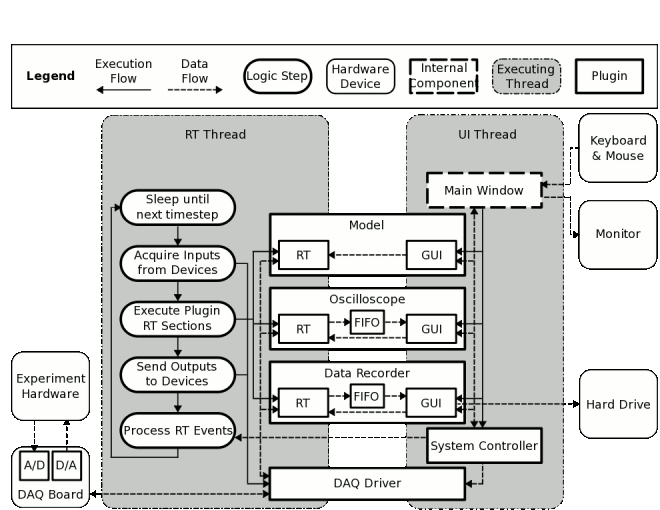
\includegraphics[width=5in]{RTXI_Block_Diagram.png} 
\caption[RTXI Architecture]{RTXI has a two-thread architecture. On every cycle, the real-time thread wakes and performs standard tasks such as sampling inputs to the DAQ card and outputting any signals. It also executes the real-time code from any loaded modules, which are dynamically linked to RTXI. The real-time thread then goes to sleep until the next cycle begins. All modules span the real-time and user interface threads.} 
\end{center}
\end{maxipage}
\end{figure}

Core system modules are not derived from the \texttt{DefaultGUIModel} class, however, and there are several different ways of implementing functionality at that level.

\begin{figure} 
\begin{maxipage}
\begin{center}
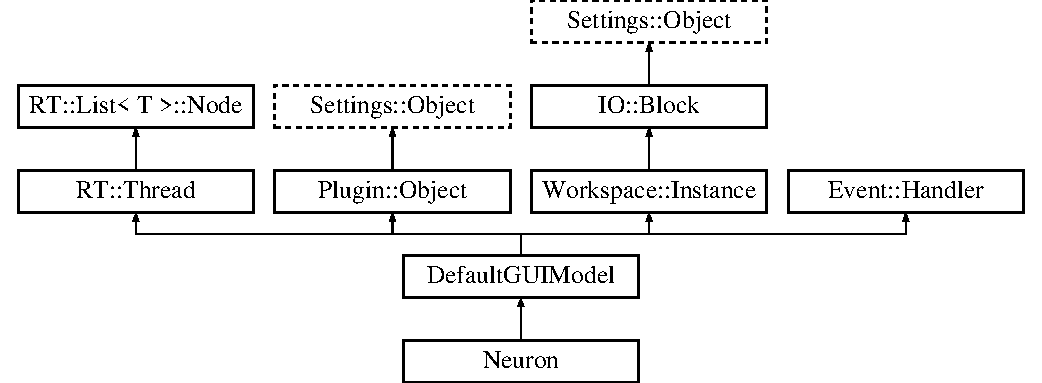
\includegraphics[width=6in]{classNeuron.pdf} 
\caption[DefaultGUIModel-derived module]{The \texttt{Neuron} module is a class derived from \texttt{DefaultGUIModel}, which inherits features such as hard real-time execution and event handling, the ability to generate and accept signals, and the ability to have metadata automatically captured by the Data Recorder to HDF5 data files.} 
\end{center}
\end{maxipage}
\end{figure}

%%%%%%%%%%%%%%%%%%%%%%%%%%%%%%%%%%%%%%%%%%%%%%%%%%%%%
\subsection{Software Requirements}

RTXI is a combination of several open source software initiatives:

\begin{enumerate}

\item
Linux,

\item
the Real Time Application Interface for Linux (RTAI),

\item
COMEDI,

\item
the Qt user interface framework, and

\item
HDF5.

\end{enumerate}

\marginlabel{Linux:}Linux is a generic term referring to Unix-like computer operating systems based on the Linux kernel. Their development is one of the most prominent examples of free and open source software collaboration; typically all the underlying source code can be used, freely modified, and redistributed, both commercially and non-commercially, by anyone under licenses such as the GNU General Public License. Desktop use of Linux has become increasingly user-friendly and popular in recent years. Typically, Linux is packaged into different distributions that include the Linux kernel and all of the supporting software required to run a complete system. These distributions may include modified versions of "vanilla" Linux source code and common applications, such as the vim text editor. The RTXI Live CD and manual installation notes are based on the Ubuntu desktop distribution, which is popular with new Linux users. It features a complete desktop environment with common productivity software and GUI applications for system administration.

\marginlabel{RTAI:}RTAI (http://www.rtai.org) provides real-time extensions to the official Linux kernel to make hard real-time applications possible. This is achieved by patching the kernel and introducing additional modules to handle task scheduling, capture system interrupts, etc. This requires that the kernel be recompiled and manual installation instructions are provided here. RTAI also provides several benchmark tests for evaluating your system's real-time performance.
\bigskip

\hrule
\bigskip
RTAI is not the only option for installing a real-time Linux kernel but it is the method used by the RTXI Live CD and described in the manual installation notes. RTXI also supports the Xenomai interface.
\bigskip
\hrule
\bigskip

\marginlabel{COMEDI:}\seealso{Chapter \ref{COMEDIsupport}\\COMEDI Support}The COMEDI project develops open-source drivers, tools, and libraries for data acquisition on Linux platforms. COMEDI supports a variety of common data acquisition module boards. Most RTXI users use DAQ cards by National Instruments, but any DAQ card that is supported by COMEDI should work with RTXI. RTXI can also handle multiple DAQ cards with a simple modification to the RTXI configuration file. A list of compatible DAQ cards is available in section 2.1.2.

\marginlabel{Qt:}\seealso{Chapter \ref{Qtmodules}\\Custom GUI Modules}
Qt is a cross-platform user-interface framework distributed by Nokia and used in RTXI under the LGPL license. This framework provides classes for developing sophisticated GUIs using a signals-and-slots mechanism similar to that of RTXI modules. RTXI uses Qt v3.3.8.

\marginlabel{HDF5:}\seealso{Chapter \ref{HDF5}\\Saving Data \& \\HDF5 Files}
HDF5 is a versatile data model that can represent complex data objects and a wide variety of metadata and allows you to quickly extract subsets of data. It is incorporated into RTXI through the Data Recorder module, which streams data to a HDF5 file along with the parameters of all modules connected to the Data Recorder. You can store multi-channel experimental recordings, instrument metadata, and browse images in a single file, making it possible to capture the entire collection of information about a single experiment. The format is completely portable and several tools are available for interacting with data in this format. HDFView is a free visual tool for browsing and editing HDF5 data structures and is available for Windows, Mac and Linux. MATLAB also has native functions for working with HDF5 files and we provide a tool that optimizes HDF5 files produced by RTXI for importing into MATLAB. We have developed a standardized hierarchical structure that will allow you to write MATLAB scripts that are compatible with all RTXI-generated HDF5 files.

RTXI depends on several additional Linux libraries that are typically available through the software repositories for each popular distribution of Linux:
\index{dependencies, software}
\begin{enumerate}
\item GNU Scientific Library (GSL)
\item Boost libraries
\item Qt 3.3.8
\item HDF5
\end{enumerate}

%%%%%%%%%%%%%%%%%%%%%%%%%%%%%%%%%%%%%%%%%%%%%%%%%%%%%
\subsection{Development Roadmap}
\label{roadmap}